% Options for packages loaded elsewhere
\PassOptionsToPackage{unicode}{hyperref}
\PassOptionsToPackage{hyphens}{url}
\PassOptionsToPackage{dvipsnames,svgnames,x11names}{xcolor}
%
\documentclass[
  article]{jss}

\usepackage{amsmath,amssymb}
\usepackage{iftex}
\ifPDFTeX
  \usepackage[T1]{fontenc}
  \usepackage[utf8]{inputenc}
  \usepackage{textcomp} % provide euro and other symbols
\else % if luatex or xetex
  \usepackage{unicode-math}
  \defaultfontfeatures{Scale=MatchLowercase}
  \defaultfontfeatures[\rmfamily]{Ligatures=TeX,Scale=1}
\fi
\usepackage{lmodern}
\ifPDFTeX\else  
    % xetex/luatex font selection
\fi
% Use upquote if available, for straight quotes in verbatim environments
\IfFileExists{upquote.sty}{\usepackage{upquote}}{}
\IfFileExists{microtype.sty}{% use microtype if available
  \usepackage[]{microtype}
  \UseMicrotypeSet[protrusion]{basicmath} % disable protrusion for tt fonts
}{}
\makeatletter
\@ifundefined{KOMAClassName}{% if non-KOMA class
  \IfFileExists{parskip.sty}{%
    \usepackage{parskip}
  }{% else
    \setlength{\parindent}{0pt}
    \setlength{\parskip}{6pt plus 2pt minus 1pt}}
}{% if KOMA class
  \KOMAoptions{parskip=half}}
\makeatother
\usepackage{xcolor}
\setlength{\emergencystretch}{3em} % prevent overfull lines
\setcounter{secnumdepth}{-\maxdimen} % remove section numbering
% Make \paragraph and \subparagraph free-standing
\ifx\paragraph\undefined\else
  \let\oldparagraph\paragraph
  \renewcommand{\paragraph}[1]{\oldparagraph{#1}\mbox{}}
\fi
\ifx\subparagraph\undefined\else
  \let\oldsubparagraph\subparagraph
  \renewcommand{\subparagraph}[1]{\oldsubparagraph{#1}\mbox{}}
\fi


\providecommand{\tightlist}{%
  \setlength{\itemsep}{0pt}\setlength{\parskip}{0pt}}\usepackage{longtable,booktabs,array}
\usepackage{calc} % for calculating minipage widths
% Correct order of tables after \paragraph or \subparagraph
\usepackage{etoolbox}
\makeatletter
\patchcmd\longtable{\par}{\if@noskipsec\mbox{}\fi\par}{}{}
\makeatother
% Allow footnotes in longtable head/foot
\IfFileExists{footnotehyper.sty}{\usepackage{footnotehyper}}{\usepackage{footnote}}
\makesavenoteenv{longtable}
\usepackage{graphicx}
\makeatletter
\def\maxwidth{\ifdim\Gin@nat@width>\linewidth\linewidth\else\Gin@nat@width\fi}
\def\maxheight{\ifdim\Gin@nat@height>\textheight\textheight\else\Gin@nat@height\fi}
\makeatother
% Scale images if necessary, so that they will not overflow the page
% margins by default, and it is still possible to overwrite the defaults
% using explicit options in \includegraphics[width, height, ...]{}
\setkeys{Gin}{width=\maxwidth,height=\maxheight,keepaspectratio}
% Set default figure placement to htbp
\makeatletter
\def\fps@figure{htbp}
\makeatother

\usepackage{orcidlink,thumbpdf,lmodern}

\newcommand{\class}[1]{`\code{#1}'}
\newcommand{\fct}[1]{\code{#1()}}
\makeatletter
\@ifpackageloaded{tcolorbox}{}{\usepackage[skins,breakable]{tcolorbox}}
\@ifpackageloaded{fontawesome5}{}{\usepackage{fontawesome5}}
\definecolor{quarto-callout-color}{HTML}{909090}
\definecolor{quarto-callout-note-color}{HTML}{0758E5}
\definecolor{quarto-callout-important-color}{HTML}{CC1914}
\definecolor{quarto-callout-warning-color}{HTML}{EB9113}
\definecolor{quarto-callout-tip-color}{HTML}{00A047}
\definecolor{quarto-callout-caution-color}{HTML}{FC5300}
\definecolor{quarto-callout-color-frame}{HTML}{acacac}
\definecolor{quarto-callout-note-color-frame}{HTML}{4582ec}
\definecolor{quarto-callout-important-color-frame}{HTML}{d9534f}
\definecolor{quarto-callout-warning-color-frame}{HTML}{f0ad4e}
\definecolor{quarto-callout-tip-color-frame}{HTML}{02b875}
\definecolor{quarto-callout-caution-color-frame}{HTML}{fd7e14}
\makeatother
\makeatletter
\makeatother
\makeatletter
\makeatother
\makeatletter
\@ifpackageloaded{caption}{}{\usepackage{caption}}
\AtBeginDocument{%
\ifdefined\contentsname
  \renewcommand*\contentsname{Table of contents}
\else
  \newcommand\contentsname{Table of contents}
\fi
\ifdefined\listfigurename
  \renewcommand*\listfigurename{List of Figures}
\else
  \newcommand\listfigurename{List of Figures}
\fi
\ifdefined\listtablename
  \renewcommand*\listtablename{List of Tables}
\else
  \newcommand\listtablename{List of Tables}
\fi
\ifdefined\figurename
  \renewcommand*\figurename{Figure}
\else
  \newcommand\figurename{Figure}
\fi
\ifdefined\tablename
  \renewcommand*\tablename{Table}
\else
  \newcommand\tablename{Table}
\fi
}
\@ifpackageloaded{float}{}{\usepackage{float}}
\floatstyle{ruled}
\@ifundefined{c@chapter}{\newfloat{codelisting}{h}{lop}}{\newfloat{codelisting}{h}{lop}[chapter]}
\floatname{codelisting}{Listing}
\newcommand*\listoflistings{\listof{codelisting}{List of Listings}}
\makeatother
\makeatletter
\@ifpackageloaded{caption}{}{\usepackage{caption}}
\@ifpackageloaded{subcaption}{}{\usepackage{subcaption}}
\makeatother
\makeatletter
\makeatother
\ifLuaTeX
  \usepackage{selnolig}  % disable illegal ligatures
\fi
\IfFileExists{bookmark.sty}{\usepackage{bookmark}}{\usepackage{hyperref}}
\IfFileExists{xurl.sty}{\usepackage{xurl}}{} % add URL line breaks if available
\urlstyle{same} % disable monospaced font for URLs
\hypersetup{
  pdftitle={Imputation of Incomplete Multilevel Data with R},
  pdfauthor={Hanne I. Oberman; Johanna Muñoz; Valentijn M.T. de Jong; Gerko Vink; Thomas P.A. Debray},
  pdfkeywords={missing data, multilevel, clustering, mice, R},
  colorlinks=true,
  linkcolor={blue},
  filecolor={Maroon},
  citecolor={Blue},
  urlcolor={Blue},
  pdfcreator={LaTeX via pandoc}}

%% -- Article metainformation (author, title, ...) -----------------------------

%% Author information
\author{Hanne I. Oberman~\orcidlink{0000-0003-3276-2141}\\Utrecht
University \And Johanna
Muñoz~\orcidlink{0000-0002-2384-5415}\\University Medical Center
Utrecht \AND Valentijn M.T. de
Jong~\orcidlink{0000-0001-9921-3468}\\University Medical Center
Utrecht \And Gerko Vink~\orcidlink{0000-0001-9767-1924}\\University
Medical Center Utrecht \AND Thomas P.A.
Debray~\orcidlink{0000-0002-1790-2719}\\University Medical Center
Utrecht}
\Plainauthor{Hanne I. Oberman, Johanna Muñoz, Valentijn M.T. de
Jong, Gerko Vink, Thomas P.A. Debray} %% comma-separated

\title{Imputation of Incomplete Multilevel Data with R}
\Plaintitle{Imputation of Incomplete Multilevel Data with
R} %% without formatting

%% an abstract and keywords
\Abstract{This tutorial illustrates the imputation of incomplete
multilevel data with the \proglang{R} packackage \pkg{mice}. Our scope
is only simple multilevel models, to show how imputation can yield less
biased estimates from incomplete clustered data. More complex models can
be accomodated, but are outside the scope of this paper. Incomplete
multilevel data requires careful consideration of the missing data
problem and analysis strategy. In this tutorial, we focus on a popular
strategy for accommodating missingness in multilevel data: replacing the
missing data with one or more plausible values, i.e.,
imputation.Imputation separates the missing data problem from the main
analysis and the completed data can be analyzed as if it has been fully
observed. This tutorial illustrates the imputation of incomplete
multilevel data with the statistical programming language R. We aim to
show how imputation can yield less biased estimates from incomplete
clustered data. We provide practical guidelines and code snippets for
different missing data situations, including non-ignorable missingness
mechanisms. For brevity, we focus on multilevel imputation using chained
equations with the R mice package and its adjacent packages.}

%% at least one keyword must be supplied
\Keywords{missing
data, multilevel, clustering, \pkg{mice}, \proglang{R}}
\Plainkeywords{missing data, multilevel, clustering, mice, R}

%% publication information
%% NOTE: Typically, this can be left commented and will be filled out by the technical editor
%% \Volume{50}
%% \Issue{9}
%% \Month{June}
%% \Year{2012}
%% \Submitdate{2012-06-04}
%% \Acceptdate{2012-06-04}
%% \setcounter{page}{1}
%% \Pages{1--xx}

%% The address of (at least) one author should be given
%% in the following format:
\Address{
Hanne I. Oberman\\
Methodology and Statistics\\
Padualaan 14\\
Utrecht The Netherlands\\
E-mail: \email{h.i.oberman@uu.nl}\\
URL: \url{https://www.hanneoberman.github.io}\\
\\~
Johanna Muñoz\\
Julius Centre for Health Sciences and Primary Care\\
Universiteitsweg 100\\
Utrecht The Netherlands\\
\\~
Valentijn M.T. de Jong\\
Julius Centre for Health Sciences and Primary Care\\
Utrecht The Netherlands\\
\\~
Gerko Vink\\
Julius Centre for Health Sciences and Primary Care\\
Universiteitsweg 100\\
Utrecht The Netherlands\\
\\~
Thomas P.A. Debray\\
Julius Centre for Health Sciences and Primary Care\\
Universiteitsweg 100\\
Utrecht The Netherlands\\
\\~

}

\begin{document}
\maketitle
\hypertarget{sec-intro}{%
\section{Introduction: Clustering and incomplete data}\label{sec-intro}}

\begin{enumerate}
\def\labelenumi{\arabic{enumi}.}
\tightlist
\item
  missing data occur often in data with human subjects
\item
  missing data may be resolved, but need to be handled in accordance
  with the analysis of scientific interest
\item
  in human-subjects research, there is often clustering, which may be
  captured with multilevel modeling techniques
\item
  if the analysis of scientific interest is a multilevel model, the
  missing data handling method should accommodate the multilevel
  structure of the data
\item
  both missingness and multilevel structures require advanced
  statistical techniques
\item
  this tutorial sets out to facilitate empirical researchers in
  accommodating both multilevel structures as well as missing data.
\item
  we illustrate the use of the software by means of three case studies
  from the social and biomedical sciences.
\end{enumerate}

\begin{verbatim}
Warning: package 'ggplot2' was built under R version 4.3.2
\end{verbatim}

\hypertarget{overview-of-software}{%
\subsection{overview of software}\label{overview-of-software}}

The popular \pkg{mice} package in \proglang{R} \citet{R}

\hypertarget{scope}{%
\subsection{scope}\label{scope}}

This papers serves as a tutorial for imputing incomplete multilevel data
with \pkg{mice} in \proglang{R}. \pkg{mice} has become the de-facto
standard for imputation by chained equations, which iteratively solves
the missingness on a variable-by-variable basis. \pkg{mice} is known to
yield valid inferences under many different missing data circumstances
\citep{buur18}.

We provide practical guidelines and code snippets for different missing
data situations, including non-ignorable mechanisms. For reasons of
brevity, we focus on multilevel imputation by chained equations with
\pkg{mice} exclusively; other imputation methods and packages \citep[see
e.g.][ and \citet{grun18}]{audi18} are outside the scope of this
tutorial. Assumed knowledge includes basic familiarity with the
\pkg{lme4} notation for multilevel models (see Table \ref{tab:mod}).

We illustrate imputation of incomplete multilevel data using three case
studies:

\begin{itemize}
\tightlist
\item
  \texttt{popmis} from the \pkg{mice} package \citep[simulated data on
  perceived popularity, \(n = 2,000\) pupils across \(N = 100\) schools
  with data that are MAR,][]{mice};
\item
  \texttt{impact} from the \pkg{metamisc} package \citep[empirical data
  on traumatic brain injuries, \(n = 11,022\) patients across \(N = 15\)
  studies with data that are MAR,][]{metamisc};
\item
  \texttt{obesity} from the \pkg{micemd} package {[}simulated data on
  obesity, \(n = 2,111\) patients across \(N = 5\) regions with data
  that are MNAR{]}.
\end{itemize}

For each of these datasets, we discuss the nature of the missingness,
choose one or more imputation models and evaluate the imputed data, but
we will also highlight one specific aspect of the imputation workflow.

This tutorial is dedicated to readers who are unfamiliar with multiple
imputation. More experienced readers can skip the introduction (case
study 1) and directly head to practical applications of multilevel
imputation under MAR conditions (case study 2) or under MNAR conditions
(case study 3).

\hypertarget{sec-models}{%
\section{Background}\label{sec-models}}

\hypertarget{concepts-in-multilevel-data}{%
\subsection{concepts in multilevel
data}\label{concepts-in-multilevel-data}}

Many datasets include individuals that are clustered together, for
example in geographic regions, or even different studies. In the
simplest case, individuals (e.g., students) are nested within a single
cluster (e.g., school classes). More complex clustered structures may
occur when there are multiple hierarchical levels (e.g., students in
different schools or patients within hospitals within regions across
countries), or when the clustering is non-nested (e.g., electronic
health record data from diverse settings and populations within large
databases). With clustered data we generally assume that individuals
from the same cluster tend to be more similar than individuals from
other clusters. In statistical terms, this implies that observations
from the same cluster are not independent and may in fact be correlated.
If this correlation is left unaddressed, estimates of \emph{p} values,
confidence intervals even model parameters are prone to bias
\citep{loca01}. Statistical methods for clustered data typically adopt
hierarchical models that explicitly describe the grouping of
observations. These models are also known as `multilevel models',
`hierarchical models', `mixed effect models', `random effect models',
and in the context of time-to-event data as `frailty models'. Table
\ref{tab:clus} provides an overview of some key concepts in multilevel
modeling.

\begin{tcolorbox}[enhanced jigsaw, arc=.35mm, bottomrule=.15mm, toprule=.15mm, breakable, leftrule=.75mm, left=2mm, colback=white, opacityback=0, rightrule=.15mm]

Box 1. The intraclass correlation coefficient.

\end{tcolorbox}

In \proglang{R}, multilevel models may be fitted using the package
\pkg{lme4}. For linear mixed-effects models, the function

\begin{verbatim}
lmer(formula, data, ...)
\end{verbatim}

\hypertarget{concepts-in-missing-data}{%
\subsection{concepts in missing data}\label{concepts-in-missing-data}}

missing data mechanisms etc.

As with any other dataset, clustered datasets may be impacted by
missingness in much the same way. Several strategies can be used to
handle missing data, including complete case analysis and imputation. We
focus on the latter approach and discuss statistical methods for
replacing the missing data with one or more plausible values. Imputation
separates the missing data problem from the analysis and the completed
data can be analyzed as if it were completely observed. It is generally
recommended to impute the missing values more than once to preserve
uncertainty due to missingness and to allow for valid inferences (c.f.
Rubin 1976).

With incomplete clustered datasets we can distinguish between two types
of missing data: sporadic missingness and systematic missingness
\citep{resc13}. Sporadic missingness arises when variables are missing
for some but not all of the units in a cluster \citep{buur18, jola18}.
For example, it is possible that test results are missing for several
students in one or more classes. When all observations are missing
within one or more clusters, data are said to be systematically missing.
Sporadic missingness is visualized in Figure XYZ.

\begin{verbatim}
plot_na()
\end{verbatim}

\begin{figure}[t]

{\centering 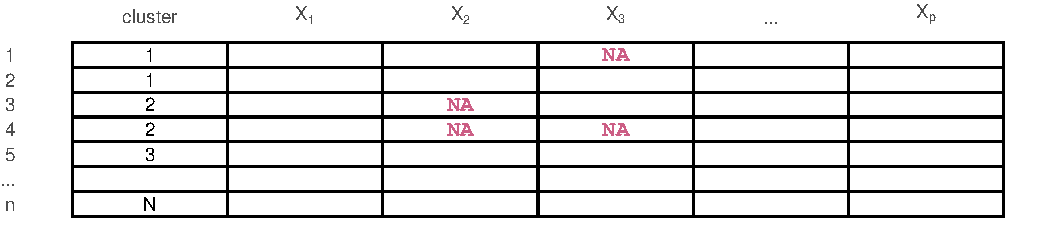
\includegraphics{manuscript_files/figure-pdf/unnamed-chunk-3-1.pdf}

}

\end{figure}

Column \(X_1\) in Figure 1 is completely observed, column \(X_2\) is
systematically missing in cluster 2, and column \(X_3\) is sporadically
missing. To analyze these incomplete data, we have to take the nature of
the missingness and the cluster structure into account. For example, the
sporadic missingness in \(X_3\) could be easily amended if this would be
a cluster-level variable (and thus constant within clusters). We could
then just extrapolate the true (but missing) value of \(X_3\) for unit 1
from unit 2, and the value for unit 4 from unit 3. If \(X_3\) would
instead be a unit-level variable (which may vary within clusters), we
could not just recover the unobserved `truth', but would need to use
some kind of missing data method, or discard the incomplete units
altogether (i.e., complete case analysis). Complete case analysis can
however introduce bias in statistical inferences and lowers statistical
power. Further, with the systematic missingness in \(X_2\), it would be
impossible to fit a multilevel model without accommodating the
missingness in some way. Complete case analysis in that case would mean
excluding the entire cluster from the analyses. The wrong choice of
missing data handling method can thus be extremely harmful to the
inferences.

Imputation of missing data requires consideration of the mechanism
behind the missingness. Rubin proposed to distinguish between data that
are missing completely at random (MCAR), data that are missing at random
(MAR) and data that are missing not at random (MNAR; see Table
\ref{tab:miss}). For each of these three missingness generating
mechanisms, different imputation strategies are warranted
(\citet{yuce08} and \citet{hox15}). We here consider the general case
that data are MAR, and expand on certain MNAR situations.

\hypertarget{imputation-with-mice}{%
\subsection{imputation with mice}\label{imputation-with-mice}}

The \proglang{R} package \pkg{mice} provides a framework for imputing
incomplete data on a variable-by-variable basis. The \fct{mice} function
allows users to flexibly specify how many times and under what model the
missing data should be imputed. This is reflected in the first four
function arguments

\begin{verbatim}
mice(data, m, method, predictorMatrix, ...)
\end{verbatim}

where \texttt{data} refers to the incomplete dataset, \texttt{m}
determines the number of imputations, \texttt{method} denotes the
functional form of the imputation model and \texttt{predictorMatrix}
specifies the interrelational dependencies between variables and
imputation models (i.e., the set of predictors to be used for imputing
each incomplete variable).

\begin{tcolorbox}[enhanced jigsaw, arc=.35mm, bottomrule=.15mm, toprule=.15mm, breakable, leftrule=.75mm, left=2mm, colback=white, opacityback=0, rightrule=.15mm]

Box 2. The \texttt{methods}.

\end{tcolorbox}

\begin{tcolorbox}[enhanced jigsaw, arc=.35mm, bottomrule=.15mm, toprule=.15mm, breakable, leftrule=.75mm, left=2mm, colback=white, opacityback=0, rightrule=.15mm]

Box 3. The predictor matrix. The entries corresponding to the level-1
predictors are coded with a 3, indicating that both the original values
as well as the cluster means of the predictor are included into the
imputation model. The entry of 4 in the predictor matrix adds three
variables to the imputation model for the imputation model predictor:
the value of the predictor, the cluster means of the predictor and the
random slopes of the predictor.

\end{tcolorbox}

\hypertarget{sec-illustrations}{%
\section{Illustrations}\label{sec-illustrations}}

In this section, we demonstrate the workflow using three case studies.

\hypertarget{setup}{%
\subsection{Setup}\label{setup}}

\begin{verbatim}
R> set.seed(123)
R> library(mice)
R> library(ggmice)
R> library(ggplot2)
R> library(miceadds)
R> library(lme4)
R> library(mitml)
R> library(broom.mixed)
\end{verbatim}

\hypertarget{popularity-data}{%
\subsection{Popularity data}\label{popularity-data}}

\begin{verbatim}
R> data("popmis", package = "mice")
\end{verbatim}

\begin{verbatim}
R> dat <- popmis[, c("school", "teachpop", "popular", "texp", "sex")] 
\end{verbatim}

\begin{verbatim}
ggmice(dat, aes(popular, teachpop)) + 
  geom_jitter()
\end{verbatim}

\begin{figure}[t]

{\centering 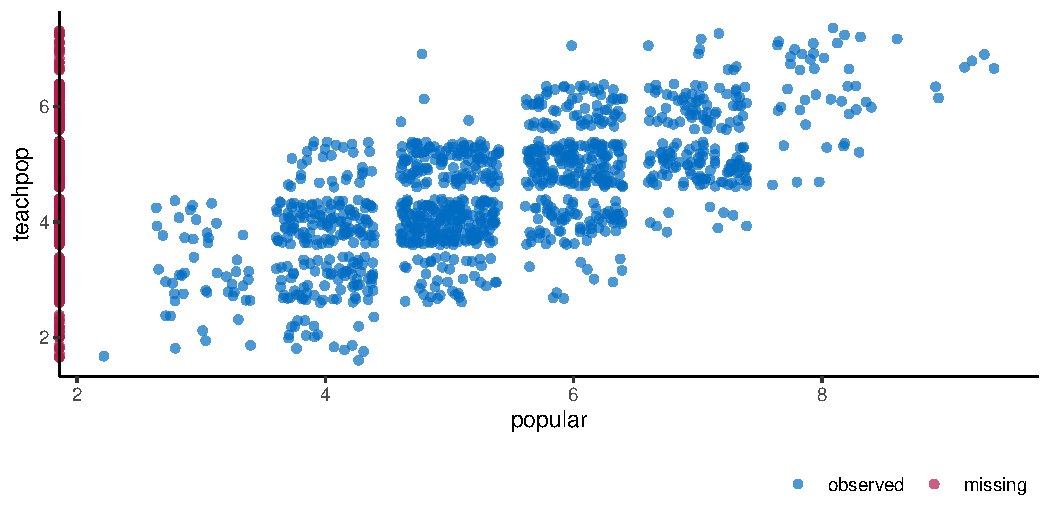
\includegraphics{manuscript_files/figure-pdf/unnamed-chunk-7-1.pdf}

}

\caption{Polar axis plot}

\end{figure}

With the \texttt{ggmice} unction \texttt{plot\_pattern} we can visualize
this.

\begin{verbatim}
R> plot_pattern(dat)
\end{verbatim}

\begin{figure}[t]

{\centering 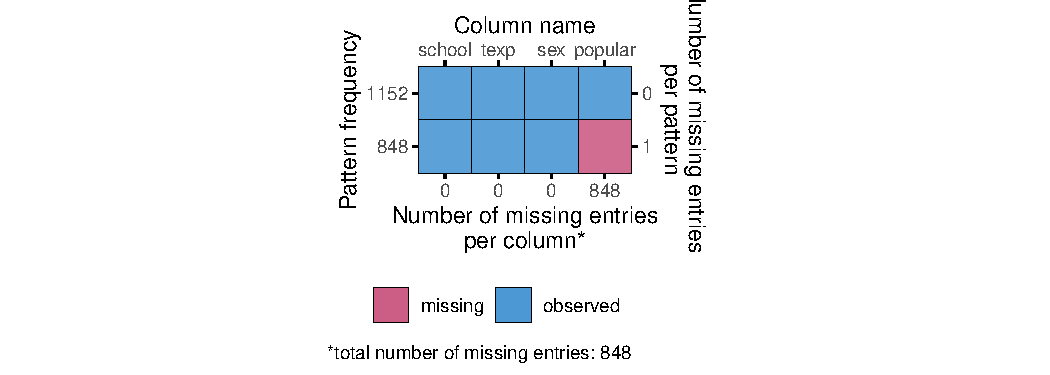
\includegraphics{manuscript_files/figure-pdf/fig-pattern-1.pdf}

}

\caption{\label{fig-pattern}Missing data pattern.}

\end{figure}

\begin{figure}

\end{figure}

\begin{verbatim}
R> plot_corr(dat)
\end{verbatim}

\begin{figure}[t]

{\centering 
\includegraphics{manuscript_files/figure-pdf/unnamed-chunk-10-1.pdf}

}

\caption{Pair-wise correlations.}

\end{figure}

\begin{verbatim}
R> meth <- make.method(dat)
R> meth
\end{verbatim}

\begin{verbatim}
  school teachpop  popular     texp      sex 
      ""       ""    "pmm"       ""       "" 
\end{verbatim}

\begin{verbatim}
R> pred <- quickpred(dat)
R> pred
\end{verbatim}

\begin{verbatim}
         school teachpop popular texp sex
school        0        0       0    0   0
teachpop      0        0       0    0   0
popular       0        1       0    1   1
texp          0        0       0    0   0
sex           0        0       0    0   0
\end{verbatim}

Adjust the methods vector.

\begin{verbatim}
R> meth["popular"] <- "2l.pmm"
\end{verbatim}

Adjust the predictor matrix.

\begin{verbatim}
R> pred["popular", "school"] <- -2
R> pred["popular", "sex"] <- 2
\end{verbatim}

Visualize the imputation methods and predictors.

\begin{verbatim}
plot_pred(pred, method = meth)
\end{verbatim}

\begin{figure}[t]

{\centering 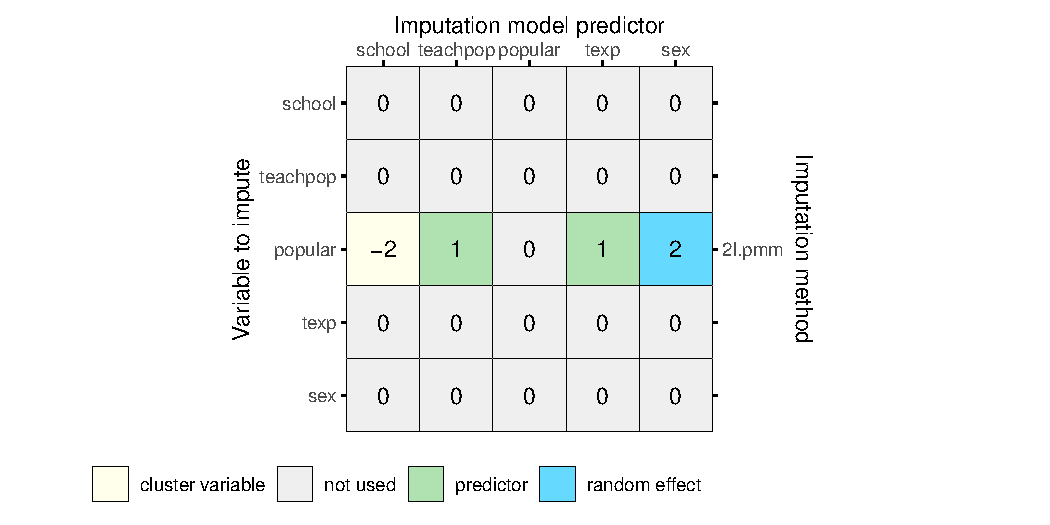
\includegraphics{manuscript_files/figure-pdf/unnamed-chunk-15-1.pdf}

}

\end{figure}

Impute the data.

\begin{verbatim}
R> imp <- mice(
+  data = dat,
+  method = meth,
+  predictorMatrix = pred,
+  printFlag = FALSE
+)
\end{verbatim}

Evaluate the convergence.

\begin{verbatim}
R> plot_trace(imp)
\end{verbatim}

\begin{figure}[t]

{\centering 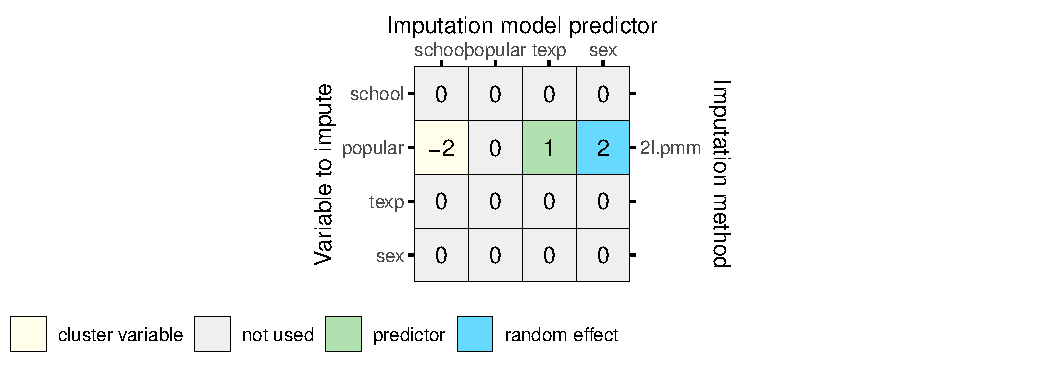
\includegraphics{manuscript_files/figure-pdf/unnamed-chunk-17-1.pdf}

}

\end{figure}

Evaluate the distribution of imputed values.

\begin{verbatim}
ggmice(imp, aes(popular, group = .imp)) + 
  geom_density() 
\end{verbatim}

\begin{figure}[t]

{\centering 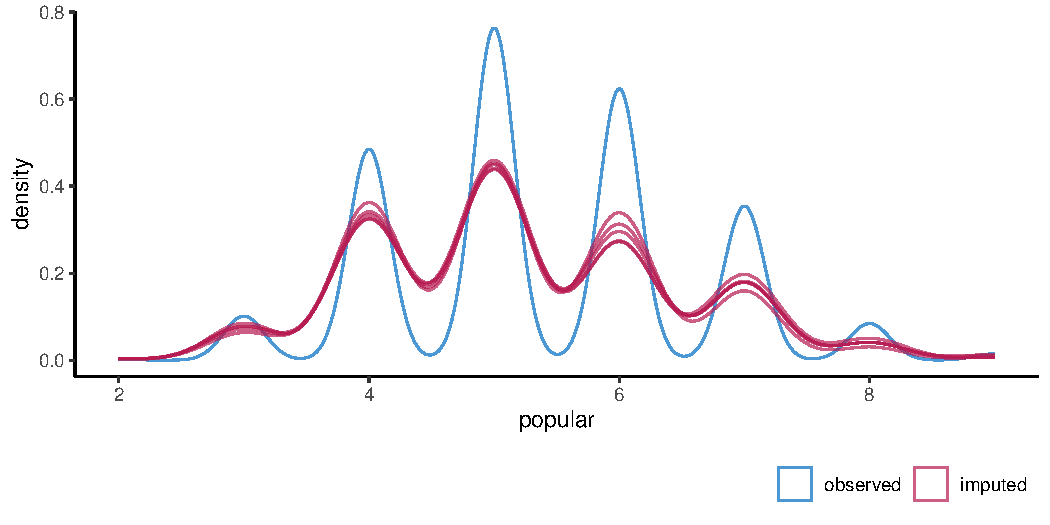
\includegraphics{manuscript_files/figure-pdf/unnamed-chunk-18-1.pdf}

}

\end{figure}

Evaluate the distribution of imputed values.

\begin{verbatim}
ggmice(imp, aes(.imp, popular)) + 
  geom_jitter(alpha = 0.05) +
    geom_boxplot()
\end{verbatim}

\begin{figure}[t]

{\centering 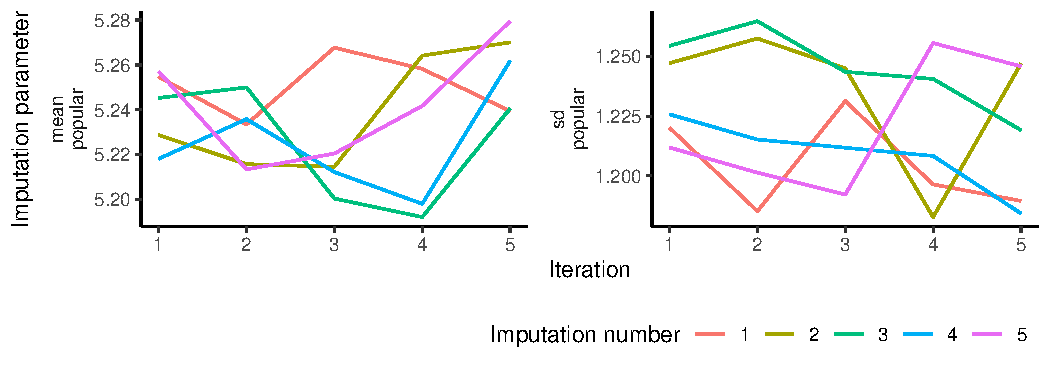
\includegraphics{manuscript_files/figure-pdf/unnamed-chunk-19-1.pdf}

}

\end{figure}

\begin{verbatim}
ggmice(imp, aes(popular, teachpop)) + 
  geom_jitter() +
  facet_wrap(~ .imp)
\end{verbatim}

\begin{figure}[t]

{\centering 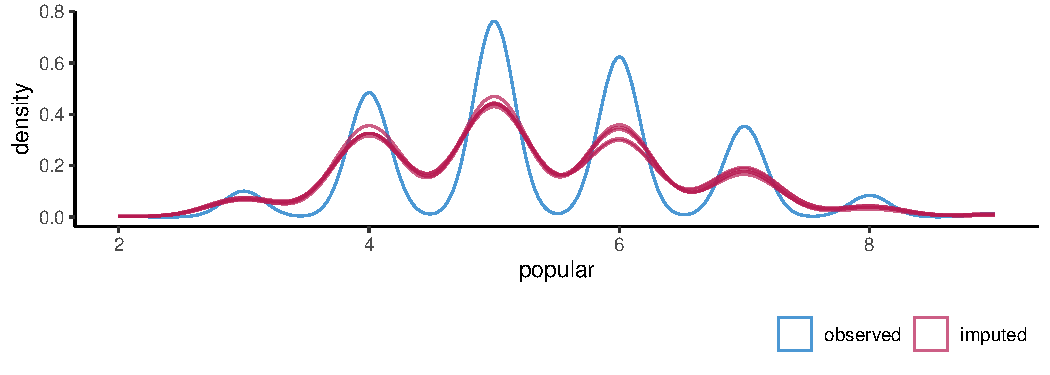
\includegraphics{manuscript_files/figure-pdf/unnamed-chunk-20-1.pdf}

}

\end{figure}

Analyze the imputed data.

\begin{verbatim}
fit <- with(
  imp,
  lmer(teachpop ~ popular + texp + (1 | school))
)
\end{verbatim}

Pool the estimates.

\begin{verbatim}
pool(fit)
\end{verbatim}

\begin{verbatim}
Class: mipo    m = 5 
         term m  estimate         ubar            b            t dfcom
1 (Intercept) 5 2.4091354 2.241304e-02 1.712964e-03 2.446860e-02  1995
2     popular 5 0.2597284 2.353344e-04 1.209648e-04 3.804922e-04  1995
3        texp 5 0.0484727 7.728295e-05 3.236252e-06 8.116646e-05  1995
         df        riv     lambda        fmi
1 432.50579 0.09171257 0.08400798 0.08821454
2  26.88403 0.61681474 0.38149995 0.42289329
3 909.68447 0.05025044 0.04784615 0.04993264
\end{verbatim}

Display results in table.

\begin{verbatim}
testEstimates(as.mitml.result(fit), extra.pars = TRUE)
\end{verbatim}

\begin{verbatim}

Call:

testEstimates(model = as.mitml.result(fit), extra.pars = TRUE)

Final parameter estimates and inferences obtained from 5 imputed data sets.

             Estimate Std.Error   t.value        df   P(>|t|)       RIV       FMI 
(Intercept)     2.409     0.156    15.401   566.786     0.000     0.092     0.087 
popular         0.260     0.020    13.315    27.483     0.000     0.617     0.422 
texp            0.048     0.009     5.380  1747.294     0.000     0.050     0.049 

                            Estimate 
Intercept~~Intercept|school    0.310 
Residual~~Residual             0.307 
ICC|school                     0.502 

Unadjusted hypothesis test as appropriate in larger samples.
\end{verbatim}

\hypertarget{sec-summary}{%
\section{Summary and discussion}\label{sec-summary}}

What is missing from this manuscript\ldots{}

\hypertarget{computational-details}{%
\section*{Computational details}\label{computational-details}}
\addcontentsline{toc}{section}{Computational details}

The results in this paper were obtained using
\proglang{R}\textasciitilde4.3.0. \proglang{R} itself and all packages
used are available from the Comprehensive \proglang{R} Archive Network
(CRAN) at {[}https://CRAN.R-project.org/{]}.

\hypertarget{acknowledgments}{%
\section*{Acknowledgments}\label{acknowledgments}}
\addcontentsline{toc}{section}{Acknowledgments}

This project has received funding from the European Union's Horizon 2020
research and innovation programme under ReCoDID grant agreement No
825746.

\hypertarget{references}{%
\section*{References}\label{references}}
\addcontentsline{toc}{section}{References}

\renewcommand{\bibsection}{}
\bibliography{bibliography.bib}

\newpage{}

\hypertarget{sec-techdetails}{%
\section*{More technical details}\label{sec-techdetails}}
\addcontentsline{toc}{section}{More technical details}

\begin{tcolorbox}[enhanced jigsaw, arc=.35mm, bottomrule=.15mm, toprule=.15mm, breakable, leftrule=.75mm, left=2mm, colback=white, opacityback=0, rightrule=.15mm]

Appendices can be included after the bibliography (with a page break).
Each section within the appendix should have a proper section title
(rather than just \emph{Appendix}).

For more technical style details, please check out JSS's style FAQ at
{[}https://www.jstatsoft.org/pages/view/style\#frequently-asked-questions{]}
which includes the following topics:

\begin{itemize}
\tightlist
\item
  Title vs.~sentence case.
\item
  Graphics formatting.
\item
  Naming conventions.
\item
  Turning JSS manuscripts into \proglang{R} package vignettes.
\item
  Trouble shooting.
\item
  Many other potentially helpful details\ldots{}
\end{itemize}

\end{tcolorbox}

\hypertarget{sec-bibtex}{%
\section*{Using BibTeX}\label{sec-bibtex}}
\addcontentsline{toc}{section}{Using BibTeX}

\begin{tcolorbox}[enhanced jigsaw, arc=.35mm, bottomrule=.15mm, toprule=.15mm, breakable, leftrule=.75mm, left=2mm, colback=white, opacityback=0, rightrule=.15mm]

References need to be provided in a \textsc{Bib}{\TeX} file
(\texttt{.bib}). All references should be made with \texttt{@cite}
syntax. This commands yield different formats of author-year citations
and allow to include additional details (e.g.,pages, chapters, \dots) in
brackets. In case you are not familiar with these commands see the JSS
style FAQ for details.

Cleaning up \textsc{Bib}{\TeX} files is a somewhat tedious task --
especially when acquiring the entries automatically from mixed online
sources. However, it is important that informations are complete and
presented in a consistent style to avoid confusions. JSS requires the
following format.

\begin{itemize}
\tightlist
\item
  item JSS-specific markup (\texttt{\textbackslash{}proglang},
  \texttt{\textbackslash{}pkg}, \texttt{\textbackslash{}code}) should be
  used in the references.
\item
  item Titles should be in title case.
\item
  item Journal titles should not be abbreviated and in title case.
\item
  item DOIs should be included where available.
\item
  item Software should be properly cited as well. For \proglang{R}
  packages \texttt{citation("pkgname")} typically provides a good
  starting point.
\end{itemize}

\end{tcolorbox}




\end{document}
